\section{Descriptive statistic}

We have $20$ variables in our dataset of which $2$ are qualitative. The \textit{status} indicates if the country is developped or developping and the \textit{adult.mortality} feature categorize the probability of dying between $15$ and $60$ years old into five levels: very low, low, middle, high, very high. 

More generally, we can classify the different variables into several categories: \textit{economic} (country status, expenditure on health, gdp, hdi), \textit{social} (total population of each country, number of years of schooling), \textit{mortality} (adult mortality, infant death, under five death, under four death because of HIV/AIDS, thinness) and \textit{immunization} factors (immunization of hepatitis b, polia, diphteria as well as number of reported cases of measles). We will only describe some variables, the curious reader can find a complete description of these in the appendix.

The \textit{hepatitis.b}, \textit{polio} and \textit{diphteria} variables are respectively the immunization coverages against hepatitis B, polio and DPT3 (diphteria tetanus toxoid and pertussis) among the $1$ year olds and are given in percentage.

The \textit{alcohol} variable is the consumption of alcohol per capita (of $15$ years old or more) in litres of pure alcohol.

\subsection{Qualitative variables}

\begin{figure}[H]
	\centering
	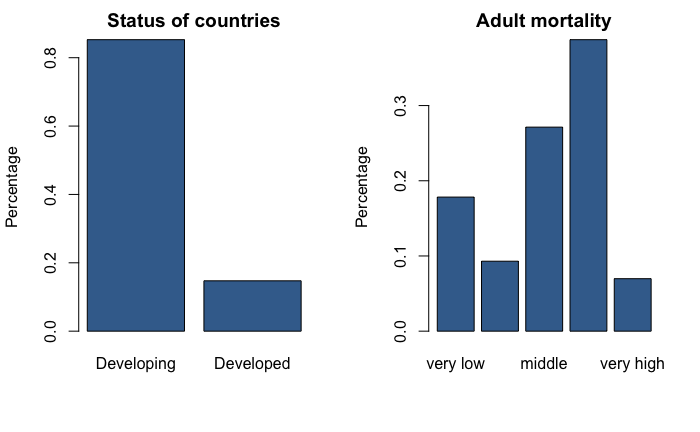
\includegraphics{figures/eda/histogram_qualitative_variables.png.png}
	\caption{barplot of the qualitative variables}
	\label{fig:qualitative_variables_barplot}
\end{figure}

\subsection{Quantitative variables}

Let's take a look to the table of the 4 moments (\textit{mean}, \textit{standard deviation}, \textit{skewness} and \textit{kurtosis}) for each of the quantitative variables. 

\begin{figure}[H]
	\centering
	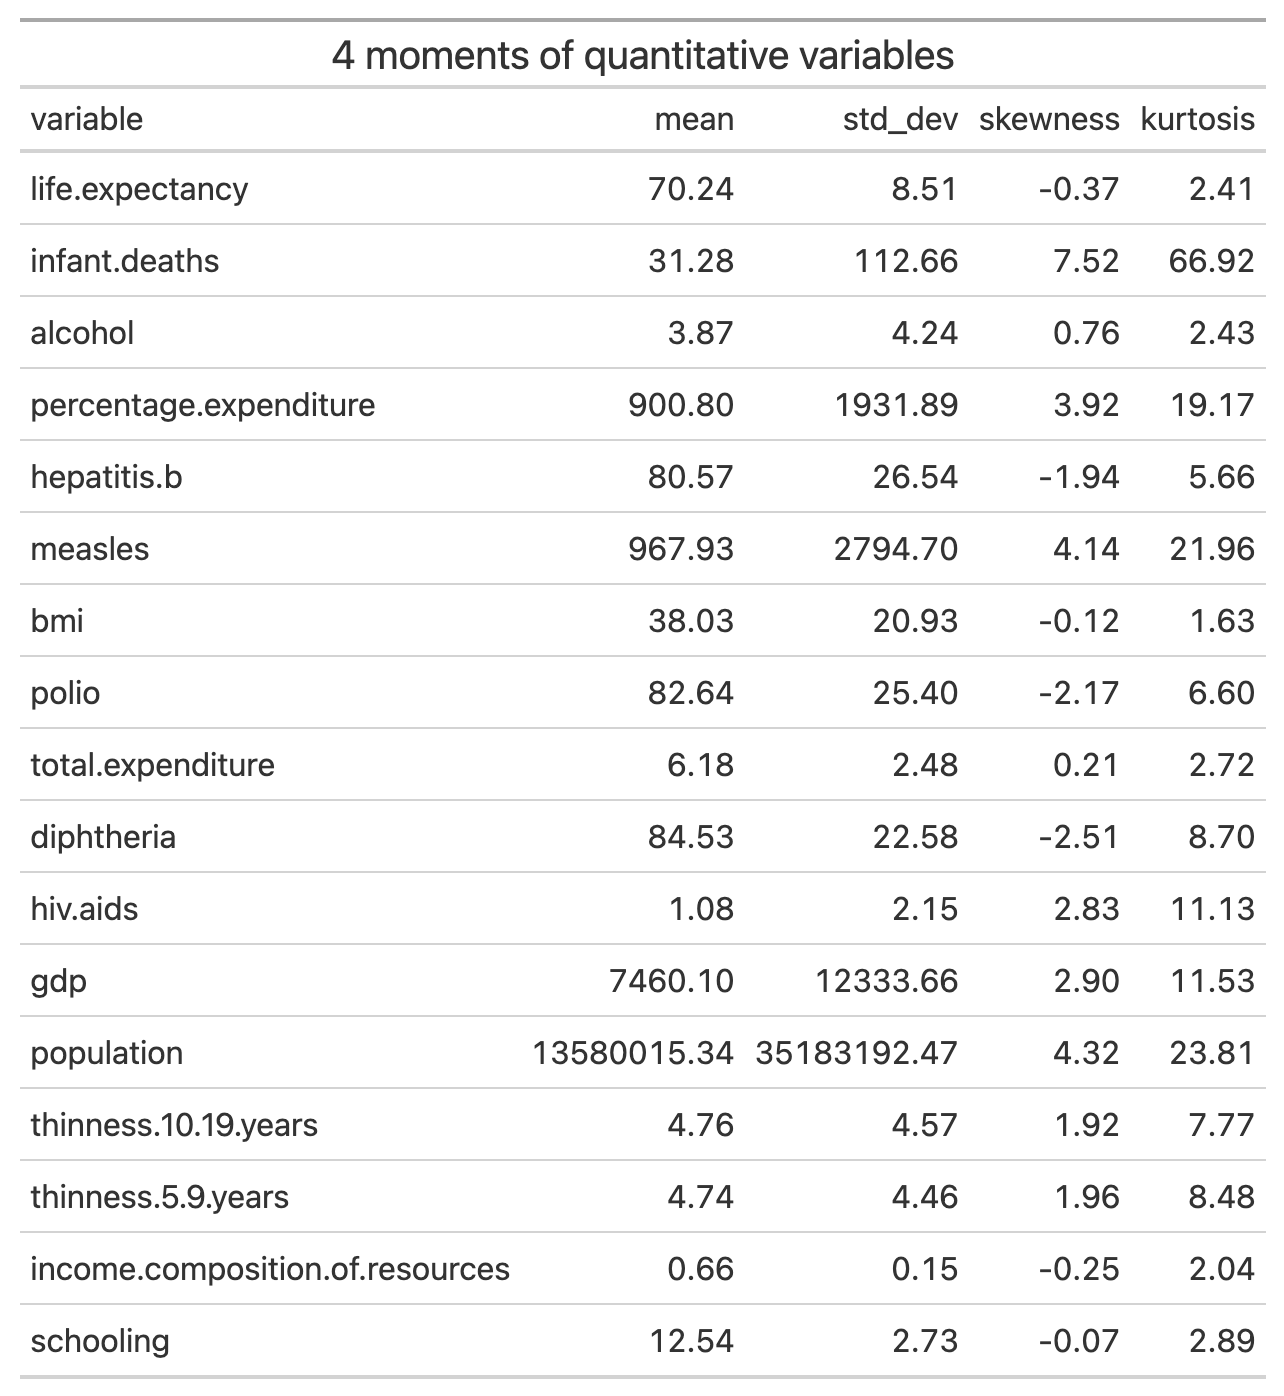
\includegraphics{figures/eda/quantitative_variables_moments.png}
	\caption{table of moments (mean, standard deviation, skewness, kurtosis) for the quantitative variables}
	\label{fig:quantitative_variables_moments}
\end{figure}

The \textbf{life expectancy} has a mean of roughly $70$ years with a standard deviation of $8.6$. It is slightly negatively skewed which indicates that some countries have low life expectancy. The kurtosis is less than $3$ so the distribution is a litlle bit flattened.

% TARGET

\begin{figure}[H]
	\centering
	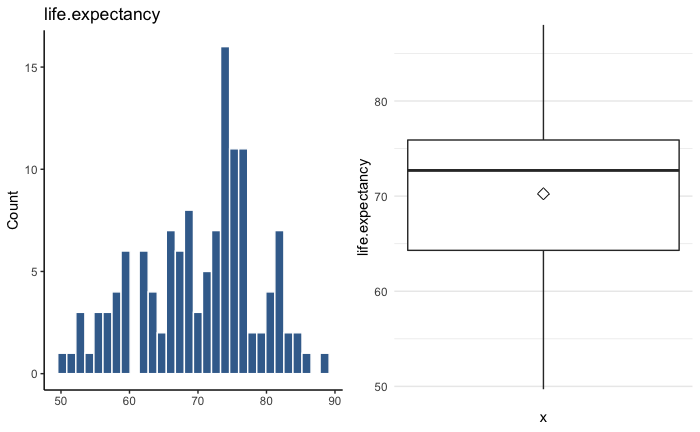
\includegraphics{figures/eda/histogram_boxplot_target.png}
	\caption{Histogram and boxplot of the target variable (life expectancy)}
	\label{fig:histogram_boxplot_target}
\end{figure}

% ECONOMIC

\begin{figure}[H]
	\centering
	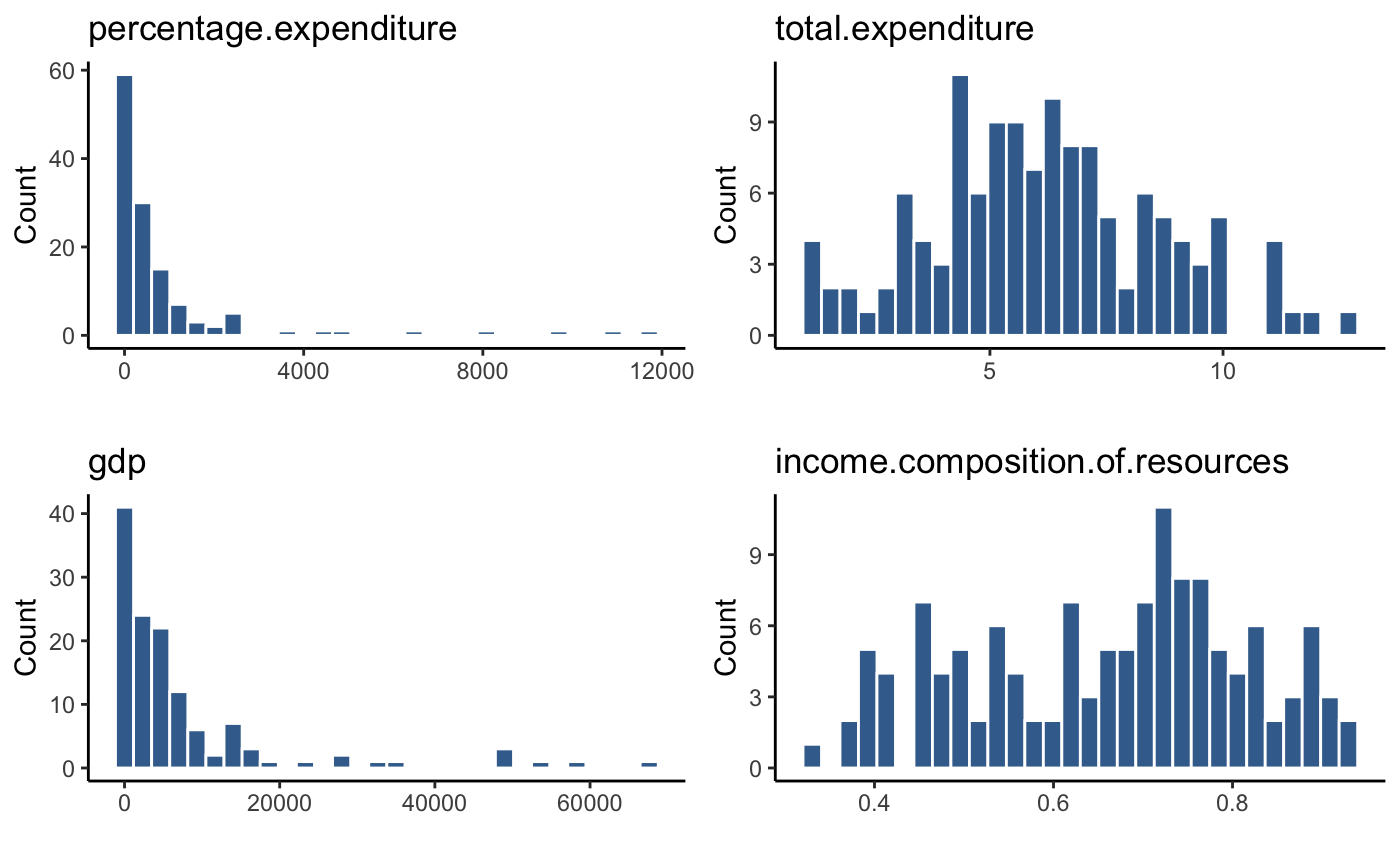
\includegraphics{figures/eda/histogram_economic_features.png}
	\caption{Histogram of economic features}
	\label{fig:histogram_economic_features}
\end{figure}

\begin{figure}[H]
	\centering
	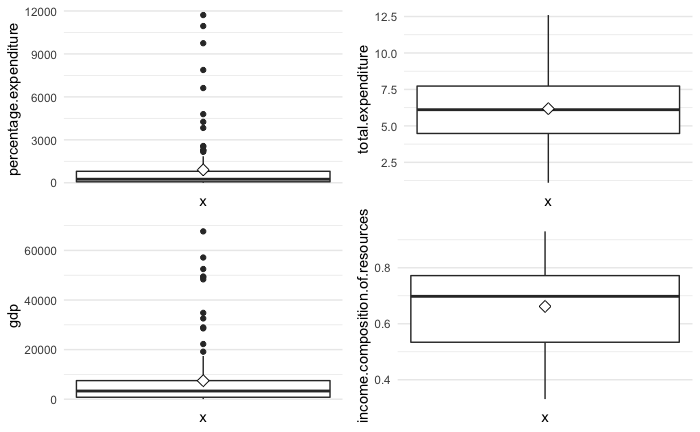
\includegraphics{figures/eda/boxplot_economic_features.png}
	\caption{Boxplot of economic features}
	\label{fig:boxplot_economic_features}
\end{figure}

% SOCIAL

\begin{figure}[H]
	\centering
	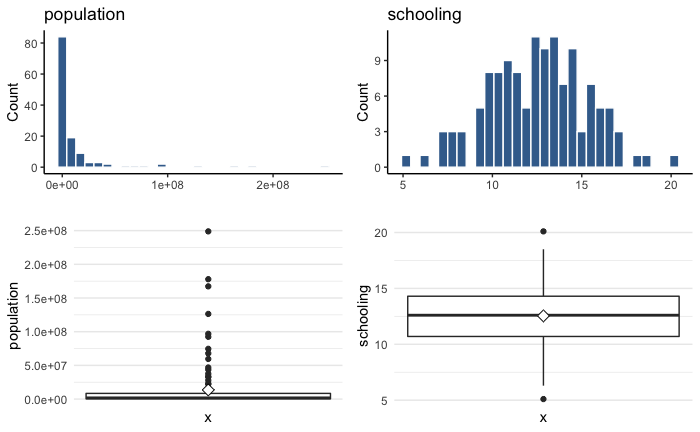
\includegraphics{figures/eda/histogram_boxplot_social_features.png}
	\caption{Histogram and boxplot of social features}
	\label{fig:histogram_boxplot_social_features}
\end{figure}

% MORTALITY

\begin{figure}[H]
	\centering
	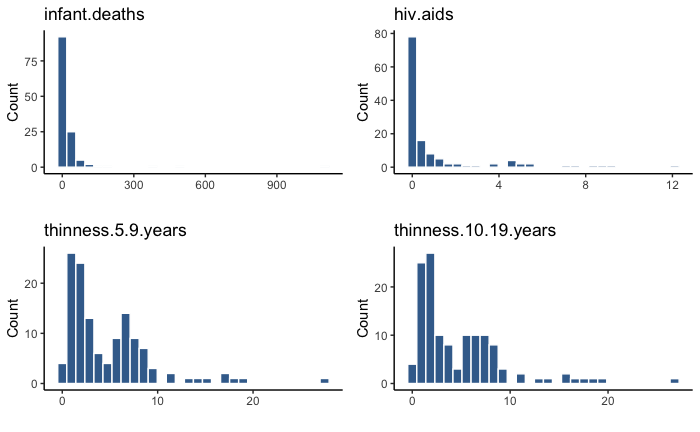
\includegraphics{figures/eda/histogram_mortality_features.png}
	\caption{Histogram of mortality features}
	\label{fig:histogram_mortality_features}
\end{figure}

\begin{figure}[H]
	\centering
	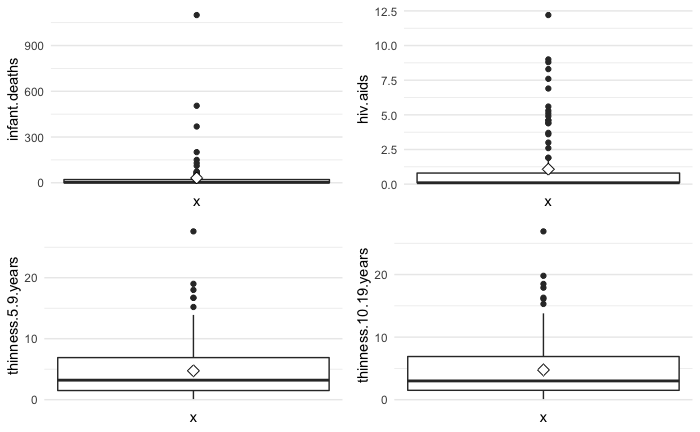
\includegraphics{figures/eda/boxplot_mortality_features.png}
	\caption{Boxplot of mortality features}
	\label{fig:boxplot_mortality_features}
\end{figure}

% HEALTH

\begin{figure}[H]
	\centering
	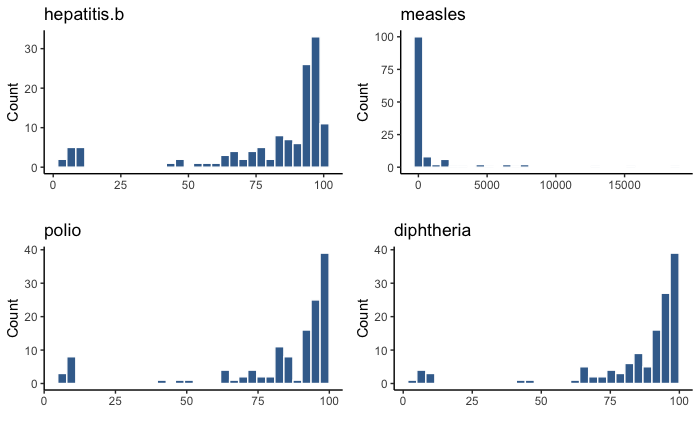
\includegraphics{figures/eda/histogram_health_features.png}
	\caption{Histogram of health features}
	\label{fig:histogram_health_features}
\end{figure}

\begin{figure}[H]
	\centering
	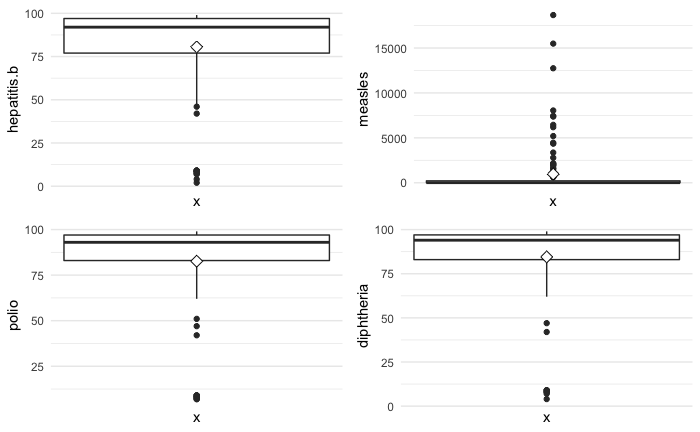
\includegraphics{figures/eda/boxplot_health_features.png}
	\caption{Boxplot of health features}
	\label{fig:boxplot_health_features}
\end{figure}

% OTHER

\begin{figure}[H]
	\centering
	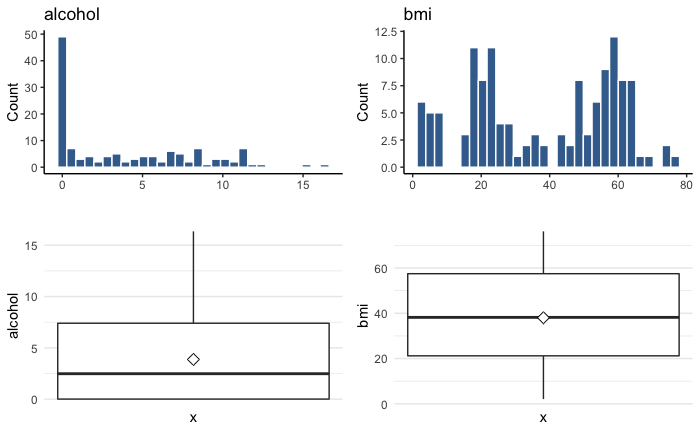
\includegraphics{figures/eda/histogram_boxplot_misc_features.png}
	\caption{Histogram and boxplot of misc features}
	\label{fig:histogram_boxplot_misc_features}
\end{figure}


The \textbf{infant death} has a mean of $31 / 1000$ but has a huge standard deviation ($112.6$). We see that heavily tailed with a kurtosis of $66.9$. The same kind of conclusion can be made for the \textbf{deaths under five year old}.

In average, countries spend $9$ times the GDP\footnote{Gross Domestic Product} per capita on health services but the standard deviation is huge ($1931.8$) which indicates the presence of outliers far away from the mean. Therefore, we expect that some countries spend much less than that on health services.

Furthermore, in average, countries spend $6 \%$ of their total budget on health services. The distribution of this variable seems to follow a normal distribution given the skewness and kurtosis.

\subsection{Correlation matrix}

We look at the correlation matrix in order to see if there are any highly correlated variables. Indeed, it could be a sign of multicollinearity

\begin{figure}[H]
	\centering
	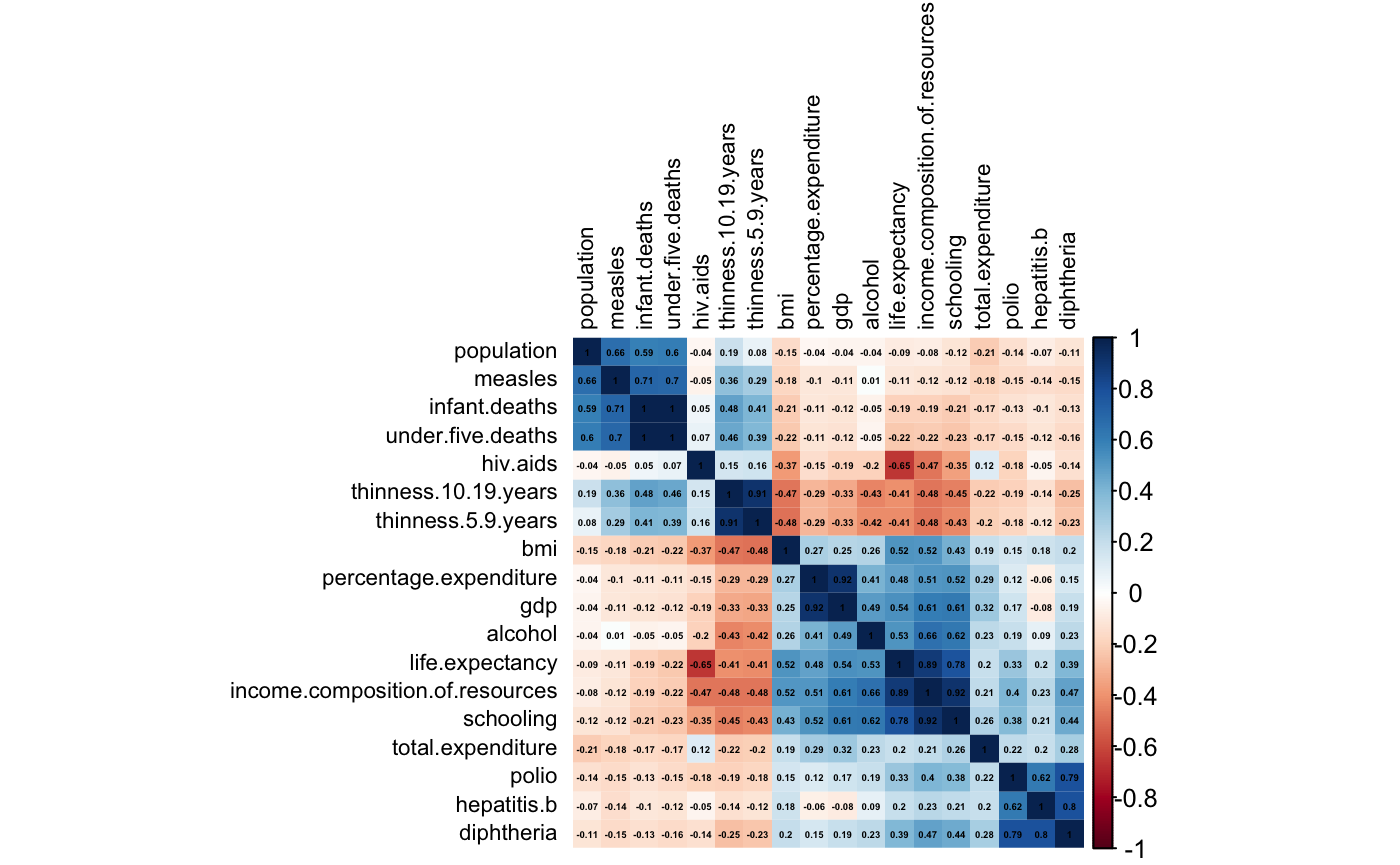
\includegraphics{figures/eda/correlation_matrix.png}
	\caption{correlation matrix of dataset}
	\label{fig:correlation_matrix}
\end{figure}

We see that severall variables are highly correlated:
\begin{itemize}
	\item The \textbf{infant death} is perfectly correlated with the \textbf{death under five year old}: these two features are redundant. As a consequence, we're gonna remove \textit{under.five.death} feature from our dataset.
	\item The \textbf{thinness from $5$ to $9$ years old} with the \textbf{thinness from $10$ to $19$ years old}: we could suspect that extreme thinness comes from a problem of access to food which implies that thinness doesn't stop at $10$ years old but continue throughout the teenage.
	\item The \textbf{number of measles cases per 1000 inhabitants} with the \textbf{infant death}: indeed, measle hits essentially children and youth and can (often) lead to death.
	\item The \textbf{percentage of expenditure made on health services} with the \textbf{GDP per capita}.
	\item The \textbf{hepatitis B} and \textbf{polio} with \textbf{diphteria}.
	\item The \textbf{life expectancy} with the \textbf{HDI in terms of income composition of resources} and \textbf{schooling}.
\end{itemize}